\documentclass[a4paper, 14pt]{extarticle}

\usepackage{../generalPreamble}
\usepackage{../conspectFormat}

\begin{document}
\begin{titlepage}
    {\centering
        {\bfseries
            
\includegraphics[height=8cm]{../res/logo.jpeg}\\
            Unity. Precision. Perfection.\\
            \vspace{3.5cm}
            \uppercase{Конспект лекций} \\
            по дисциплине \enquote{Конструирование ПО}\\
        }
        \vspace{\fill}
    }
    \begin{tabular}{l l}
        \textbf{Лектор}: & Спицын\\
        \textbf{Страниц}: &\pageref{LastPage}\\
        \textbf{Последнее обновление}: & \today{}\\ 
        \textbf{Автор}: & Корытов Павел, 6304\\
    \end{tabular}

    \vspace{2cm}
    {\centering
        Санкт-Петербург \\
        \the\year\\
    }
\end{titlepage}

\tableofcontents
\newpage
\section{Введение}
\subsection{Семантика и интерпретация языков программирования}
\subsubsection*{Уровни языков}
\begin{figure}[h]
    \centering
    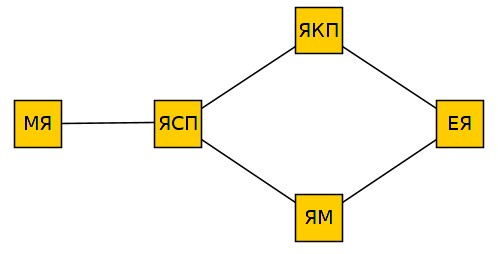
\includegraphics[width=0.7\textwidth]{./img/L1/S001.jpg}
    \caption{Уровни языков}%
    \label{img:l1:1}
\end{figure}

\begin{itemize}
    \item \dfn{МЯ} --- машинный язык
    \item \dfn{ЯСП} --- язык машинного программирования
    \item \dfn{ЯКП} --- язык конечного пользователя. Более формализованное подможество естественного языка. 
    \item \dfn{ЯН} --- язык моделирования
    \item \dfn{ЕЯ} --- естественный язык 
\end{itemize}

В процессе разработки программной системы происходит последовательный переход от описания её на ЕЯ к описанию на языках других уровней.

Переход с ЯСП на МЯ выполняется автоматически в процессе компиляции. Переходы с ЕЯ к ЯКП и ЯМ, по крайней мере в настоящий момент, не формализованы. Современные языки программирования облегчают переход с ЯКП/ЯМ к ЯСП.

При переходе с одного уровня на другой происходит потеря и приобретение семантики. Простота интерпретации примитивов языка принципиально влияет на качество разрабатываемого ПО.

Восстановить код на ЯСП по МЯ в исходном виде невозможно. Например, для C++ невозможно определить иерархию наследования по машинному коду.

Диаграмму классов в каком-то виде можно восстановить по ЯСП, но не полность. Диаграммы вроде Use Case, State UML и т.п. восстановить практически невозможно. Т.е. полноценно востановить UML по программному коду невозможно. Это связано с тем, что не все отношения, показанные на UML, реализованы в коде.

\subsubsection*{Язык}
\dfn{Язык} --- это средство коммуникации между партнерами в целях их кооперации. Для кооперации необходима общая модель мира и согласованные действия в этом мире. Поэтому, цель любого языка --- описание модели мира, описание и предписание действий в этом мире

\subsubsection*{Естественный язык}
Синтаксической и семантической единицей естественного языка является предложение. Предложения бывают:
\begin{itemize}
    \item Повелительные --- предписывают действие
    \begin{itemize}
        \item Процедурные --- описывают последовательность действий
        \item Непроцедурные --- описывают результат
    \end{itemize}
    \item Повествовательные, вопросительные --- используются для передачи личной модели мира.
\end{itemize}

С логической точки зрения, все предложения кроме повелительного процедурного типа являются предикатами. Таким образом, естественный язык можно охарактеризовать как предикативный язык с редкими процедурными вставками 

В армии общение с помощью повелительных предложений процедурного типа обеспечивает эффективность выполнения операций. В демократических представительных органах, напротив, основная цель --- передача личной модели мира. Выработка законов --- задача сложная и трудноформализуемая; только общением в таком стиле можно решить эту задачу.

\subsubsection*{Семантический разрыв}
В процессе разработки программной системы происходит переход от непроцедурного описания на естественном языке к полностью процедурной реализации на машинном языке. В результате возникает семантический разрыв между разными уровнями языков.

В лингвистике известна \textit{гипотеза Ворфа}, которая гласит, что один индивид, владеющий определённым языком, может представить себе нечто, недоступное для понимания другим индивидом, владеющим другим языком

С другой стороны, в теории чисел известен \textit{тезис Черча}, о том, что любое вычисление (алгоритм) можно реализовать на машине Тьюринга.

Применение объектно-ориентированных языков упрощает интерпретацию, поскольку можно легко получить модель предметной области в терминах объектов и классов

\subsection{Семантические уровни программной системы}
\begin{figure}[h]
    \centering
    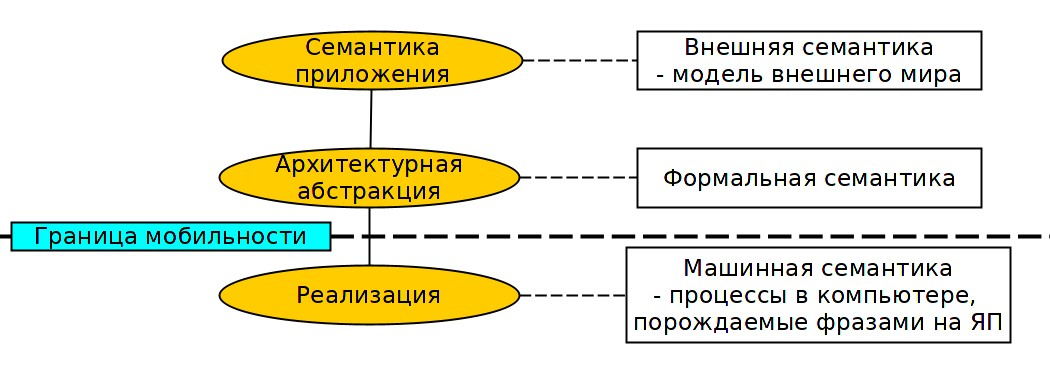
\includegraphics[width=0.8\textwidth]{./img/L1/S002.jpg}
    \caption{Уровни программной системы}%
    \label{img:l1:2}
\end{figure}

\subsubsection*{Объектный подход}
\dfn{Объект} --- всё, чем можно управлять. Он имеет \dfn{свойства}, абстрагируемый как \dfn{атрибуты}, и \dfn{поведение}, абстрагируемое в форме \dfn{методов}. 

\dfn{Тип} объекта обычно называется \dfn{классом}, класс может рассматриваться как своего рода \dfn{метаобъект}. Образуемые метаобъектами классы называются \dfn{метаклассы}

\dfn{Объекто-ориентированный анализ} --- это методология построения модели взаимодействия предметной области в терминах объектов и классов.

\dfn{Объектно-ориетированное проектирование} --- это методология, основанная на объектной декомпозиции и приемов построения физических и логических моделей

\dfn{Объекто-ориентированное программирование} --- методика программирования, основанная на представлении программы в виде сущностей (взаимодействующих объектов), каждая из которых принадлежит классам, 

\end{document}
